%%%%%%%%%%%%%%%%%%%%%%%%%%%%% SLIDE 4.0 %%%%%%%%%%%%%%%%%%%%%%%%%%%%%%%%%%%%%%%%%%%
\begin{frame}{{\bf \color{blue} Coordenadas diferenciais}}

\begin{block}{\bf Coordenadas diferenciais}
Seja uma malha triangular $\mathcal{M} = (V, E, F)$. Cada vértice $\mathbf{v}_i \in V$ possui uma representação cartesiana dada por $\mathbf{v}_i = (x_i,y_i,z_i)$.

\medskip

\destaq{Coordenadas diferenciais} (ou $\mathbf{\delta}$\textit{-coordenadas}) de $\mathbf{v}_i$ são definidas como a diferença entre a coordenada cartesiana e o centro de massa de seus vizinhos imediatos na malha:

\begin{equation}
\mathbf{\delta}_i = (\mathbf{\delta}_i^{(x)}, \mathbf{\delta}_i^{(y)}, \mathbf{\delta}_i^{(z)}) = \mathbf{v}_i - \frac{1}{d_i} \sum_{j \in N(i)} \mathbf{v}_j,
\label{eq_delta}
\end{equation}

\noindent em que $N(i) = \{j|(i,j) \in E$\} e $d_i = |N(i)|$.
\end{block}

\end{frame}

%%%%%%%%%%%%%%%%%%%%%%%%%%%%%%%%%%%%%%%%%%%%%%%%%%%%%%%%%%%%%%%%%%%%%%%%%%%%%%%
%%%%%%%%%%%%%%%%%%%%%%%%%%%%%%%%%%%%%%%%%%%%%%%%%%%%%%%%%%%%%%%%%%%%%%%%%%%%%%%

\begin{frame}{{\bf \color{blue} Pesos nas $\delta$-coordenadas}}
\begin{block}{\bf $\delta$-coordenadas ponderadas}
Adicionando pesos às arestas $E$, é possível alterar o relacionamento entre um vértice e cada um de seus vizinhos.

\medskip

Assim, as alterações a um vértice irão se propagar a cada um dos vizinhos deste de forma proporcional ao peso da aresta entre eles.

\medskip

$$\delta_i = c_i \sum_{j \in N(i)} w_{ij} (v_i - v_j)$$
\end{block}
\end{frame}

\begin{frame}{{\bf \color{blue} Pesos nas $\delta$-coordenadas}}
\begin{block}{\bf Ponderação padrão: média dos vizinhos}
$$\delta_i = \frac{1}{d_i} \sum_{j \in N(i)} (v_i - v_j)$$

O peso de todas as arestas é constante e $\mathbf{c_i}$ depende unicamente do número de vizinhos de $\mathbf{v_i}$. Desta forma, alterações sofridas por um vértice são distribuídas uniformemente entre os vértices vizinhos a ele.
\end{block}
\end{frame}

\begin{frame}{{\bf \color{blue} Pesos nas $\delta$-coordenadas}}
\begin{block}{\bf Pesos cotangentes}
Recomendáveis para malhas muito irregulares, gera apenas componentes normais.

$$\mathbf{\delta}_i^c = \frac{1}{|\Omega|} \sum_{j \in N(i)} \frac{1}{2} (\cot \alpha_{ij} + \cot \beta_{ij})(\mathbf{v}_i - \mathbf{v}_j))$$

\noindent em que $|\Omega|$ é o tamanho da célula de Voronoi de $i$ e $\alpha_{ij}, \beta_{ij}$ são os dois ângulos opostos à aresta $(i, j)$.
\end{block}
\end{frame}

\begin{frame}[fragile]{{\bf \color{blue} Coordenadas diferenciais}}
\begin{Codigo}[geração das $\delta$-coordenadas]
\noindent\rule{11.2cm}{1.pt}
\vspace{-0.2cm}
\begin{verbatim}
	
function [ delta ] = geraDeltaCoords(v, w, c)
 % geraDeltaCoords: Gera as delta-coordenadas
 %   Gera as coords dif. a partir das absolutas e pesos w e c
 % Entrada
 %   v: vetor contendo as n (x, y, z) coordenadas;
 %   w, c: pesos de cada adjacência w(i, j) e de cada vértice
 %       delta_i = c_i * sum_j (w_ij * (v_i - v_j))
 [n, x] = size(v); % número de [vertices, dimensão]
 delta = zeros(n, x);
 for i=1:n
  for j=1:n
   delta(i,:) = delta(i,:) + w(i,j) * (v(i,:) - v(j,:));
  end
  delta(i,:) = c(i) * delta(i,:);
 end
end
\end{verbatim}\\
\vspace{-0.5cm}
\noindent\rule{11.2cm}{1.pt}\\
\end{Codigo}	
\end{frame}

%%%%%%%%%%%%%%%%%%%%%%%%%%%%% SLIDE 4.0 %%%%%%%%%%%%%%%%%%%%%%%%%%%%%%%%%%%%%%%%%%%
\begin{frame}{{\bf \color{blue} Transformação para $\delta$-coordenadas}}
	
\begin{block}{\bf Matriz transformação para $\delta$-coordenadas}
	Seja $A$ a matriz de adjacências da malha:
	
	$$
	A_{ij} = \begin{cases}
	1&(i, j) \in E\\
	0&\text{caso contrário.}
	\end{cases}
	$$
	
	e $D$ a matriz diagonal tal que
	
	$$D_{ii} = d_{i} = |N(i)| = \text{número de vértices adjacentes a }i$$
	
	A matriz $L$ de transformação de coordenadas cartesianas para as coordenadas diferenciais é:
	
	\begin{equation}
	L = I - D^{-1}A.
	\end{equation}
	
\end{block}
	
\end{frame}



%%%%%%%%%%%%%%%%%%%%%%%%%%%%% SLIDE 4.0 %%%%%%%%%%%%%%%%%%%%%%%%%%%%%%%%%%%%%%%%%%%
\begin{frame}{{\bf \color{blue} Transformação para $\delta$-coordenadas}}

\begin{block}{\bf Matriz simétrica de transformação}
	É mais comum utilizar a versão simétrica de $L$, $L_s$, tal que:
	
	$$L_s = DL = D - A$$
	
	e cada célula pode ser calculada por:
	
	\begin{equation}
	(L_s)_{ij} = \begin{cases}
	d_i&i=j\\
	-1&(i, j) \in E\\
	0&\text{caso contrário.}
	\end{cases}
	\end{equation}
	
\end{block}

\end{frame}


%%%%%%%%%%%%%%%%%%%%%%%%%%%%% SLIDE 4.0 %%%%%%%%%%%%%%%%%%%%%%%%%%%%%%%%%%%%%%%%%%%
\begin{frame}{{\bf \color{blue} Transformação para $\delta$-coordenadas}}
	
\begin{block}{\bf Matriz simétrica de transformação}
Temos:

$$L_s \textbf{x} = \delta^{(x)}$$
$$L_s \textbf{y} = \delta^{(y)}$$
$$L_s \textbf{z} = \delta^{(z)}$$

e $L_s$ é denominado o \destaq{Laplaciano topológico} da malha $\mathcal M$.
	
\end{block}

\end{frame}


\begin{frame}[fragile]{{\bf \color{blue} Matriz laplaciana}}
\begin{Codigo}[geração do Laplaciano topológico $L_s$]
\noindent\rule{11.2cm}{1.pt}
\vspace{-0.2cm}
\begin{verbatim}
function [ Ls ] = geraLaplaciano(adj)
 % geraLaplaciano Gera a matriz simetrica do laplaciano
 %   Gera a matriz simétrica do Laplaciano Topológico
 % Entrada:
 %   adj: matriz de adjacências da malha original
 n = size(adj, 1); % número de vértices
 D = diag(sum(adj));
 Ls = D - adj; % Laplaciano simétrico L_s
end
\end{verbatim}\\
\vspace{-0.5cm}
\noindent\rule{11.2cm}{1.pt}\\
\end{Codigo}
\end{frame}


%%%%%%%%%%%%%%%%%%%%%%%%%%%%% SLIDE 4.0 %%%%%%%%%%%%%%%%%%%%%%%%%%%%%%%%%%%%%%%%%%%
\begin{frame}{{\bf \color{blue} Discretização de Laplace-Beltrami}}
	
\begin{block}{\bf Discretização de Laplace-Beltrami}
Se considerar $\mathcal{M}$ uma aproximação linear por partes de uma superfície suave,

$$\delta_i = \frac{1}{d_i} \sum_{j \in N(i)}(\mathbf{v_i} - \mathbf{v_j})$$

é uma discretização de

$$\frac{1}{|\gamma|} \int_{v \in \gamma} (v_i - v) dl(v)$$

em que $\gamma$ é uma curva de uma superfície fechada simples em volta de $v_i$ e $|\gamma|$ é o comprimento de $\gamma$.
	
\end{block}
\end{frame}


%%%%%%%%%%%%%%%%%%%%%%%%%%%%% SLIDE 4.0 %%%%%%%%%%%%%%%%%%%%%%%%%%%%%%%%%%%%%%%%%%%
\begin{frame}{{\bf \color{blue} Discretização de Laplace-Beltrami}}

\begin{block}{\bf Discretização de Laplace-Beltrami}
Sabe-se que:

$$\lim\limits_{|\gamma|\rightarrow 0} \frac{1}{|\gamma|} \int_{v \in \gamma} (v_i - v) dl(v) = -H(v_i) n_i$$

em que $H(v_i)$ é a curvatura média de $v_i$ e $n_i$ é a normal à superfície.

\medskip

Intuitivamente, as $\delta$-coordenadas \destaq{encapsulam a forma local da superfície}.
	
\end{block}
\end{frame}

%%%%%%%%%%%%%%%%%%%%%%%%%%%%%%%%%%%%%%%%%%%%%%%%%%%%%%%%%%%%%%%%%%%%%%%%%%%%%%%

\begin{frame}{{\bf \color{blue} Discretização de Laplace-Beltrami}}

\begin{block}{\bf Vantagens das $\delta$-coordenadas}
\begin{itemize}
    \item Representam detalhes locais
    \begin{itemize}
        \item A direção aproxima o vetor normal;
        \item A norma aproxima a curvatura média;
    \end{itemize}
    \medskip
    \item Utilização de matrizes esparsas (economizam tempo/memória computacionalmente).
\end{itemize}
\end{block}

\end{frame}

%%%%%%%%%%%%%%%%%%%%%%%%%%%%%%%%%%%%%%%%%%%%%%%%%%%%%%%%%%%%%%%%%%%%%%%%%%%%%%%


%%%%%%%%%%%%%%%%%%%%%%%%%%%%% SLIDE 4.0 %%%%%%%%%%%%%%%%%%%%%%%%%%%%%%%%%%%%%%%%%%%
\begin{frame}{{\bf \color{blue} Reconstrução das coordenadas cartesianas}}

\begin{block}{\bf Reconstrução das coordenadas cartesianas a partir das $\delta$-coordenadas}
$$L_s \textbf{x} = \delta^{(x)}$$

\begin{itemize}
	\item $\delta$-coordenadas são invariantes à translação;
	\item $L$ e $L_s$ são singulares;
	\item $\textbf{x} = L_s^{-1} \delta^{(x)}$ é \textbf{indefinido}.
	\item \destaq{Solução:} adicionar restrições de quem se conhece a localização.
	
\end{itemize}
\end{block}
\end{frame}


%%%%%%%%%%%%%%%%%%%%%%%%%%%%% SLIDE 4.0 %%%%%%%%%%%%%%%%%%%%%%%%%%%%%%%%%%%%%%%%%%%
\begin{frame}{{\bf \color{blue} Reconstrução das coordenadas cartesianas}}

\begin{block}{\bf Reconstrução das coordenadas cartesianas a partir das $\delta$-coordenadas}
$$L_s \textbf{x} = \delta^{(x)}$$

\begin{itemize}
	\item $rank(L) = n - k$, em que $k$ é o número de componentes;
	\item Fixar vértices $C = \{1, 2, \dots, m\}$, em que sabe-se $\{v_{C_1}, v_{C_2}, \dots, v_{C_m}\}$;
	\item Ou seja, adicionar restrições $v_{j} = c_j,\ j \in C$;
	\item Tornando o sistema \textit{full-rank}.
\end{itemize}	
\end{block}
\end{frame}


%%%%%%%%%%%%%%%%%%%%%%%%%%%%% SLIDE 4.0 %%%%%%%%%%%%%%%%%%%%%%%%%%%%%%%%%%%%%%%%%%%
\begin{frame}{{\bf \color{blue} Reconstrução das coordenadas cartesianas}}

\begin{block}{\bf Reconstrução das coordenadas cartesianas a partir das $\delta$-coordenadas}
Fixar vértices $C = \{1, \dots, m\}$ em que sabe-se $\{v_{C_1}, v_{C_2}, \dots, v_{C_m}\}$:

\bigskip

$$\left(\frac{L}{I_{m\times m} | 0}\right) \textbf{x} = \begin{pmatrix}
\delta^{(x)} \\
c_{1:m}
\end{pmatrix}$$

\medskip

E o mesmo para os outros vetores de coordenadas $\mathbf{y, z, \dots}$
\end{block}
\end{frame}

%%%%%%%%%%%%%%%%%%%%%%%%%%%%% SLIDE 4.0 %%%%%%%%%%%%%%%%%%%%%%%%%%%%%%%%%%%%%%%%%%%
\begin{frame}{{\bf \color{blue} Reconstrução das coordenadas cartesianas}}
Inicialmente, tem-se:

\bigskip

\begin{center}
	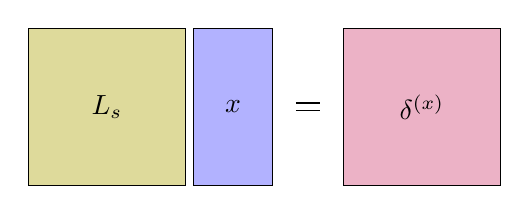
\begin{tikzpicture}
	\filldraw[fill=olive!30!white, draw=black] (0,0) rectangle node{$L_s$} (2,2);
	\filldraw[fill=blue!30!white, draw=black] (2.1,0) rectangle node{$x$} (3.1,2);
	\draw (3.4, 0.95) -- (3.7, 0.95);
	\draw (3.4, 1.05) -- (3.7, 1.05);
	\filldraw[fill=purple!30!white, draw=black] (4,0) rectangle node{$\delta^{(x)}$} (6,2);
	\end{tikzpicture}
\end{center}

\end{frame}

%%%%%%%%%%%%%%%%%%%%%%%%%%%%% SLIDE 4.0 %%%%%%%%%%%%%%%%%%%%%%%%%%%%%%%%%%%%%%%%%%%
\begin{frame}{{\bf \color{blue} Reconstrução das coordenadas cartesianas}}
Fixar vértices $C = \{1, \dots, m\}$ em que sabe-se $\{v_{C_1}, v_{C_2}, \dots, v_{C_m}\}$:

\bigskip

\begin{center}
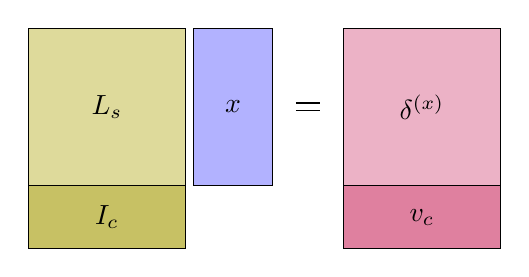
\begin{tikzpicture}
\filldraw[fill=olive!30!white, draw=black] (0,0) rectangle node{$L_s$} (2,2);
\filldraw[fill=olive!50!white, draw=black] (0,0) rectangle node{$I_c$} (2,-0.8);
\filldraw[fill=blue!30!white, draw=black] (2.1,0) rectangle node{$x$} (3.1,2);
\draw (3.4, 0.95) -- (3.7, 0.95);
\draw (3.4, 1.05) -- (3.7, 1.05);
\filldraw[fill=purple!30!white, draw=black] (4,0) rectangle node{$\delta^{(x)}$} (6,2);
\filldraw[fill=purple!50!white, draw=black] (4,0) rectangle node{$v_c$} (6,-0.8);
\end{tikzpicture}
\end{center}

\end{frame}


%%%%%%%%%%%%%%%%%%%%%%%%%%%%% SLIDE 4.0 %%%%%%%%%%%%%%%%%%%%%%%%%%%%%%%%%%%%%%%%%%%
\begin{frame}{{\bf \color{blue} Reconstrução das coordenadas cartesianas}}
Fixar vértices $C = \{1, \dots, m\}$ em que sabe-se $\{v_{C_1}, v_{C_2}, \dots, v_{C_m}\}$:

\bigskip

\begin{center}
	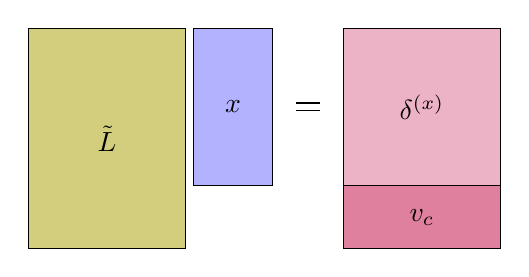
\begin{tikzpicture}
	\filldraw[fill=olive!40!white, draw=black] (0,-0.8) rectangle node{$\tilde{L}$} (2,2);
	\filldraw[fill=blue!30!white, draw=black] (2.1,0) rectangle node{$x$} (3.1,2);
	\draw (3.4, 0.95) -- (3.7, 0.95);
	\draw (3.4, 1.05) -- (3.7, 1.05);
	\filldraw[fill=purple!30!white, draw=black] (4,0) rectangle node{$\delta^{(x)}$} (6,2);
	\filldraw[fill=purple!50!white, draw=black] (4,0) rectangle node{$v_c$} (6,-0.8);
	\end{tikzpicture}
\end{center}

\end{frame}


%%%%%%%%%%%%%%%%%%%%%%%%%%%%% SLIDE 4.0 %%%%%%%%%%%%%%%%%%%%%%%%%%%%%%%%%%%%%%%%%%%
\begin{frame}{{\bf \color{blue} Reconstrução das coordenadas cartesianas}}
\begin{figure}
	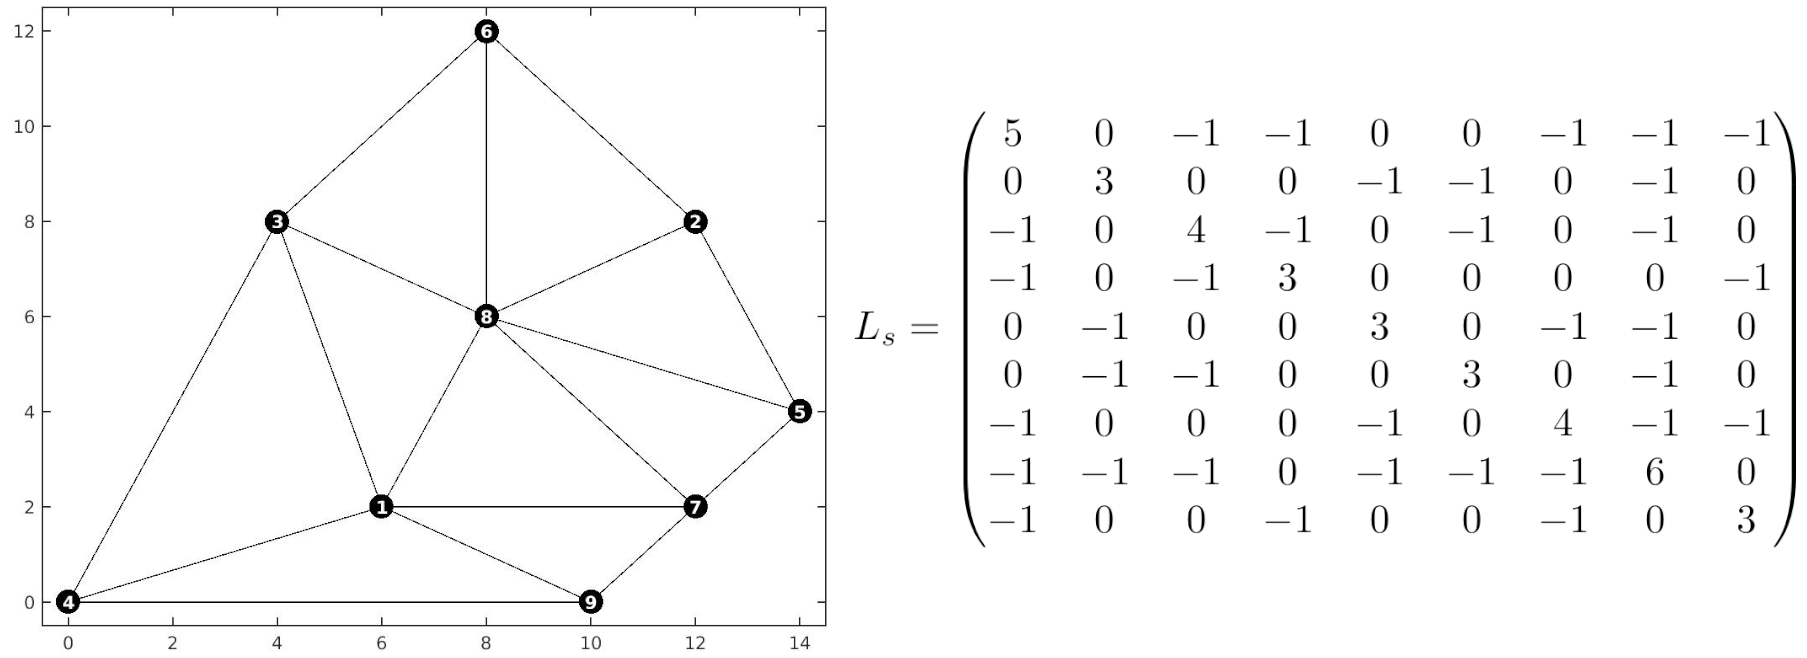
\includegraphics[width=1\linewidth]{imagens/grafo_lapl.png}
	\caption{Exemplo da matriz $L_s$}
\end{figure}
\end{frame}

\begin{frame}{{\bf \color{blue} Reconstrução das coordenadas cartesianas}}
	\begin{figure}
		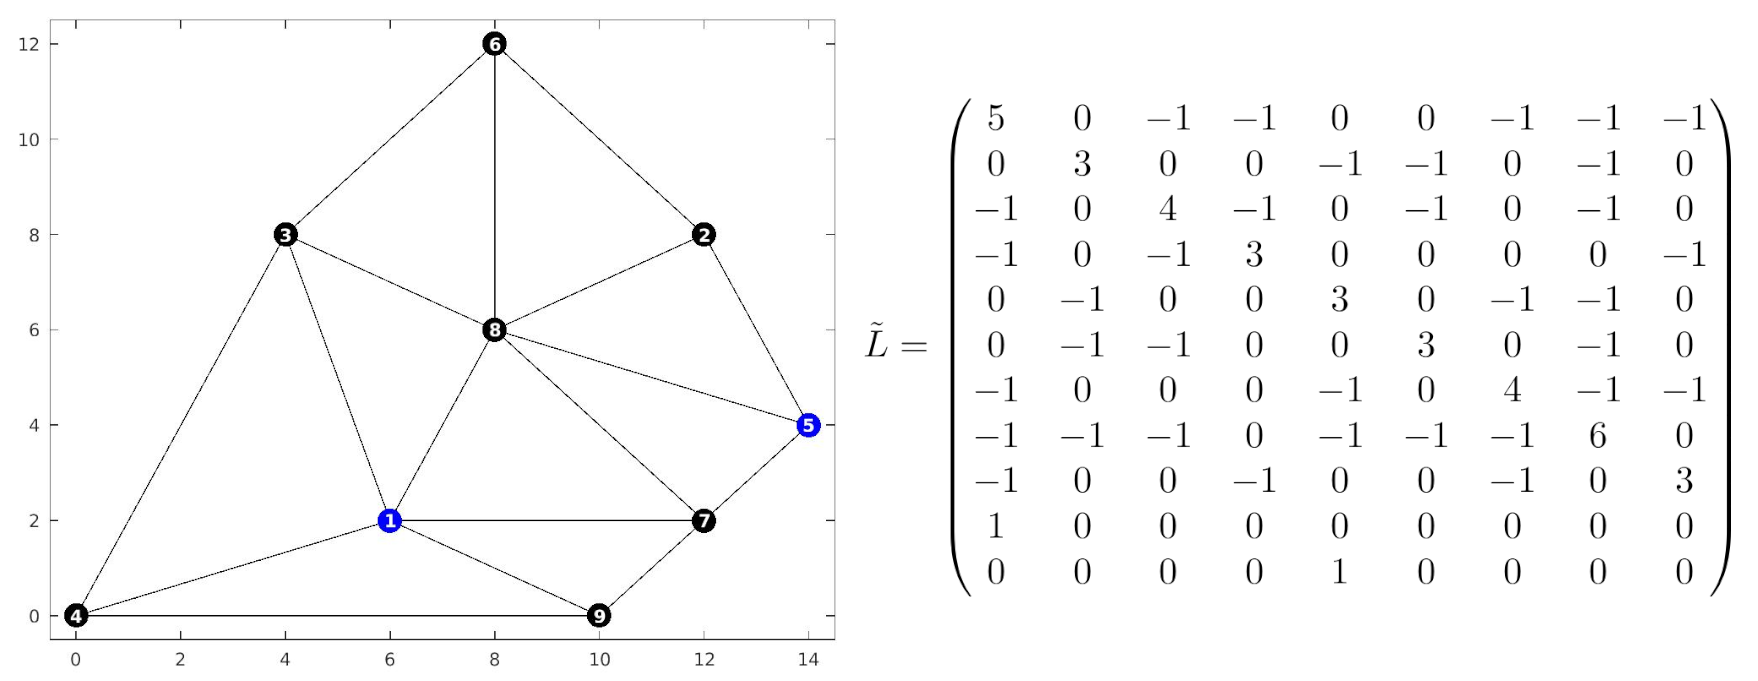
\includegraphics[width=1\linewidth]{imagens/grafo_lapl_tilde.png}
		\caption{Exemplo da matriz $\tilde{L}$ fixando os vértices 1 e 5}
	\end{figure}
\end{frame}

\begin{frame}[fragile]{{\bf \color{blue} Reconstrução das coordenadas cartesianas}}
\begin{Codigo}[recuperação das coordenadas cartesianas a partir das $\delta$-coordenadas]
\noindent\rule{11.2cm}{1.pt}
\vspace{-0.2cm}
\begin{verbatim}
n = size(L, 1); % numero de vertices
[m, x] = size(values) % numero de [vert conhecidos, dimensão]

L = [L; zeros(m, n)]; % expande L com I_mxm
delta = [delta; zeros(m, n)]; % expande Delta
for i=1:m
 L(i+n, known(1,i)) = 1;
 delta(i+n,:) = values(i,:);
end

v = []; % resolve para cada coordenada
for i=1:x
 v = [v (L \ delta(:, i))];
end
\end{verbatim}\\
\vspace{-0.5cm}
\noindent\rule{11.2cm}{1.pt}\\
\end{Codigo}
\end{frame}

\subsection{Molas e malhas dinâmicas}

\begin{frame}{{\bf \color{blue} Molas e malhas dinâmicas}}
	\begin{block}{\bf Representação de molas e malhas dinâmicas}
		Utilizando pesos, é possível simular o comportamento de molas para as arestas.
	\end{block}
	
	\begin{block}{\bf Lei de Hooke}
		Seja $F$ a força elástica exercida por uma mola, $k$ a constante de resistência específica da mola e $x$ a deformação sofrida pela mola.
		A Lei de Hooke descreve a força $F$ em função de $k$ e $x$ pela fórmula: 
		\begin{equation}
			F = -kx
		\end{equation}
	\end{block}
\end{frame}

\begin{frame}{{\bf \color{blue} Molas}}
	\begin{block}{\bf Lei de Hooke e Pesos}
		Se $k$ for inversamente proporcional à distância entre dois vértices vizinhos, $i$ e $j$, ou seja, ao tamanho da aresta entre eles, arestas mais curtas serão mais rígidas, e portanto os efeitos de uma transformação em $i$ serão refletidos mais claramente em $j$. Da mesma forma, conforme o tamanho da aresta aumenta, a propagação das alterações do vértice $i$ no vértice $j$ será menor. 
	\end{block}
\end{frame}

\begin{frame}{{\bf \color{blue} Malhas Dinâmicas}}
	
	\begin{block}{\bf Malhas Dinâmicas}
		O uso de Malhas Dinâmicas é um modelo de transformações de domínio em modelagem baseada em malhas em que não há alterações na interconectividade dos vértices, ou seja, novas arestas não são criadas e arestas existentes não são removidas. As transformações são realizadas movimentando os vértices da malha. Sendo assim, não há necessidade de remalhamento após transformações exceto em casos de deformações extremas.
	\end{block}
	
	
\end{frame}

\begin{frame}{{\bf \color{blue} Malhas Dinâmicas}}
	
	\begin{block}{\bf Criação de Malhas Dinâmicas}
		
		A criação de malhas dinâmicas consiste na distribuição de molas virtuais pela malha original. Estas molas movem os vértices vizinhos quando um vértice $i$ é manipulado, com estas transformações sendo propagadas de forma cada vez mais branda aos vértices vizinhos destes, de forma que a malha se conforme à nova descrição do domínio. Estas molas também possuem o objetivo de impedir que formas geométricas inválidas sejam criadas durante a manipulação dos vértices. 
	\end{block}
	
\end{frame}